\documentclass[12pt,aspectratio=169]{beamer}

% Input
\usepackage[utf8]{inputenc}
\usepackage[T1]{fontenc}
\usepackage[letterspace=100]{microtype}
\usepackage{upquote}

% Beamer
\usetheme{metropolis}
\usepackage[sfdefault]{FiraSans}
\usepackage{xcolor}
\definecolor{blue}{HTML}{002957}
\definecolor{red}{HTML}{F1563F}
\setbeamercolor{palette primary}{fg=white,bg=blue}
\setbeamercolor{title separator}{fg=red,bg=blue}
\setbeamercolor{frametitle}{fg=white,bg=blue}
\setbeamercolor{progress bar}{fg=red,bg=blue}
\setbeamercolor{alerted text}{fg=red,bg=blue}
\makeatletter
\setlength{\metropolis@titleseparator@linewidth}{2pt}
\setlength{\metropolis@progressonsectionpage@linewidth}{2pt}
\setlength{\metropolis@progressinheadfoot@linewidth}{2pt}
\makeatother

% Graphics
\usepackage{graphicx}
\usepackage{epstopdf}
\DeclareGraphicsExtensions{.png,.pdf,.eps}
\tikzset{
  invisible/.style={opacity=0},
  visible on/.style={alt={#1{}{invisible}}},
  alt/.code args={<#1>#2#3}{%
    \alt<#1>{\pgfkeysalso{#2}}{\pgfkeysalso{#3}} % \pgfkeysalso doesn't change the path
  },
}
\usetikzlibrary{arrows, shapes}

% Various
  %---------------------------------------------------------------------------------------
\usepackage{hyperref}
\usepackage{minted}
\usepackage{fontawesome}
\usepackage{multicol}
\usepackage[normalem]{ulem}

% No page numbers
\setbeamertemplate{footline}{}

% Title
\title{Plonen monet mahdollisuudet}
\subtitle{TIVIA Keski-Suomi}
\date{11.9.2025}
\author{Asko Soukka}

\begin{document}

%---------------------------------------------------------------------------------------

\maketitle

%---------------------------------------------------------------------------------------

\begin{frame}{Monolithic CMS}
\centering
\begin{tikzpicture}[every node/.style={font=\sffamily}]
  % Stacked CMS layers
  \node[draw, thick, fill=blue!10, minimum width=6cm, minimum height=5.1cm, label=above:{\textbf{Monolithic CMS}}] (cms) {};
  % Stacks inside CMS
  \node[draw, fill=red!10, minimum width=5.2cm, minimum height=0.7cm, anchor=north] (presentation) at ([yshift=2.1cm]cms.center) {\footnotesize Presentation};
  \node[draw, fill=red!10, minimum width=5.2cm, minimum height=1.6cm, anchor=north, align=center] (customcode) at ([yshift=1.2cm]cms.center) {\vspace{0.3cm}\footnotesize Custom Code\vspace{0.3cm}};
  \node[draw, fill=red!10, minimum width=5.2cm, minimum height=0.7cm, anchor=north] (workflows) at ([yshift=-0.6cm]cms.center) {\footnotesize Workflows};
  \node[draw, fill=red!10, minimum width=5.2cm, minimum height=0.7cm, anchor=north] (content) at ([yshift=-1.5cm]cms.center) {\footnotesize Content};
\end{tikzpicture}
\end{frame}

%---------------------------------------------------------------------------------------

\begin{frame}{Headless CMS}
\centering
\begin{tikzpicture}[every node/.style={font=\sffamily}]
  % REST API box
  \node[draw, thick, rounded corners, fill=none, minimum width=6.2cm, minimum height=3.5cm, label=above:{API}] (restapi) {};
  % Headless CMS box inside REST API
  \node[draw, thick, fill=blue!10, minimum width=4.8cm, minimum height=2.2cm, label=above:{\textbf{Headless CMS}}] (cms) at (restapi.center) {};
  % Content inside CMS
  \node[draw, fill=red!10, minimum width=3.0cm, minimum height=0.9cm] (content) at (cms.center) {\footnotesize Content};

  % External components
  \node[draw, fill=red!10, minimum width=3.5cm, minimum height=0.7cm] (presentation) at ([yshift=-1cm]restapi.south) {\footnotesize Presentation};
  \node[draw, fill=red!10, minimum width=3.5cm, minimum height=0.7cm, anchor=east] (integrations) at ([xshift=-0.5cm]restapi.west) {\footnotesize Custom Code};
  \node[draw, fill=red!10, minimum width=3.5cm, minimum height=0.7cm, anchor=west] (process) at ([xshift=0.5cm]restapi.east) {\footnotesize Workflows};

  % Bidirectional arrows (external components <-> REST API)
  \draw[<->, thick] (presentation.north) -- (restapi.south);
  \draw[<->, thick] (integrations.east) -- (restapi.west);
  \draw[<->, thick] (process.west) -- (restapi.east);
\end{tikzpicture}
\end{frame}

%---------------------------------------------------------------------------------------

\begin{frame}{Plone CMS}
  \begin{itemize}
    \item[2001] Plone 0.1: Initial public release
    \item[2003] Plone 1.0: First stable release
    \item[2007] Plone 3.0: Low code "content rules"
    \item[] \ldots
    \item[2012] Plone 4.2: Python 2.7
    \item[2013] Plone 4.3: REST API, Low code "content types"
    \item[] \ldots
    \item[2019] Plone 5.2: Python 3
    \item[2022] Plone 6.0: Headless CMS
  \end{itemize}
\end{frame}

%---------------------------------------------------------------------------------------

\begin{frame}{Plone CMS}
\centering
\begin{tikzpicture}[every node/.style={font=\sffamily}]
  % REST API box
  \node[draw, thick, rounded corners, fill=none, minimum width=6.2cm, minimum height=3.5cm, label=above:{REST API}] (restapi) {};
  % Headless CMS box inside REST API
  \node[draw, thick, fill=blue!10, minimum width=4.8cm, minimum height=2.2cm] (cms) at (restapi.center) {};
  % Content inside CMS
  \node[draw, fill=red!10, minimum width=3.0cm, minimum height=0.9cm] (content) at (cms.center) {\footnotesize Backend / Classic};

  % External components
  \node[draw, fill=red!10, minimum width=3.5cm, minimum height=0.7cm] (presentation) at ([yshift=-1cm]restapi.south) {\footnotesize Frontend / Volto};

  % Bidirectional arrows (external components <-> REST API)
  \draw[<->, thick] (presentation.north) -- (restapi.south);
\end{tikzpicture}
\end{frame}

%---------------------------------------------------------------------------------------

\begin{frame}{Workflows}
  \centering
  \begin{tikzpicture}[node distance=2.2cm, every node/.style={font=\sffamily}]
    % States (vertical layout)
    \node[draw, thick, fill=blue!10, minimum width=2.8cm, minimum height=1cm] (private) {Private};
    \node[draw, thick, fill=blue!10, minimum width=2.8cm, minimum height=1cm, below of=private] (pending) {Pending Review};
    \node[draw, thick, fill=blue!10, minimum width=2.8cm, minimum height=1cm, below of=pending] (published) {Published};

    % Transitions
    \draw[->, thick] (published) to[bend right=100] node[right] {Hide} (private);
    \draw[->, thick] (private) -- node[right=20] {Submit} (pending);
    \draw[->, thick] (pending) -- node[right=20] {Publish} (published);
    \draw[->, thick] (pending) to[bend left=100] node[left] {Retract} (private);
  \end{tikzpicture}
\end{frame}

%---------------------------------------------------------------------------------------

\begin{frame}{Rolemap}
  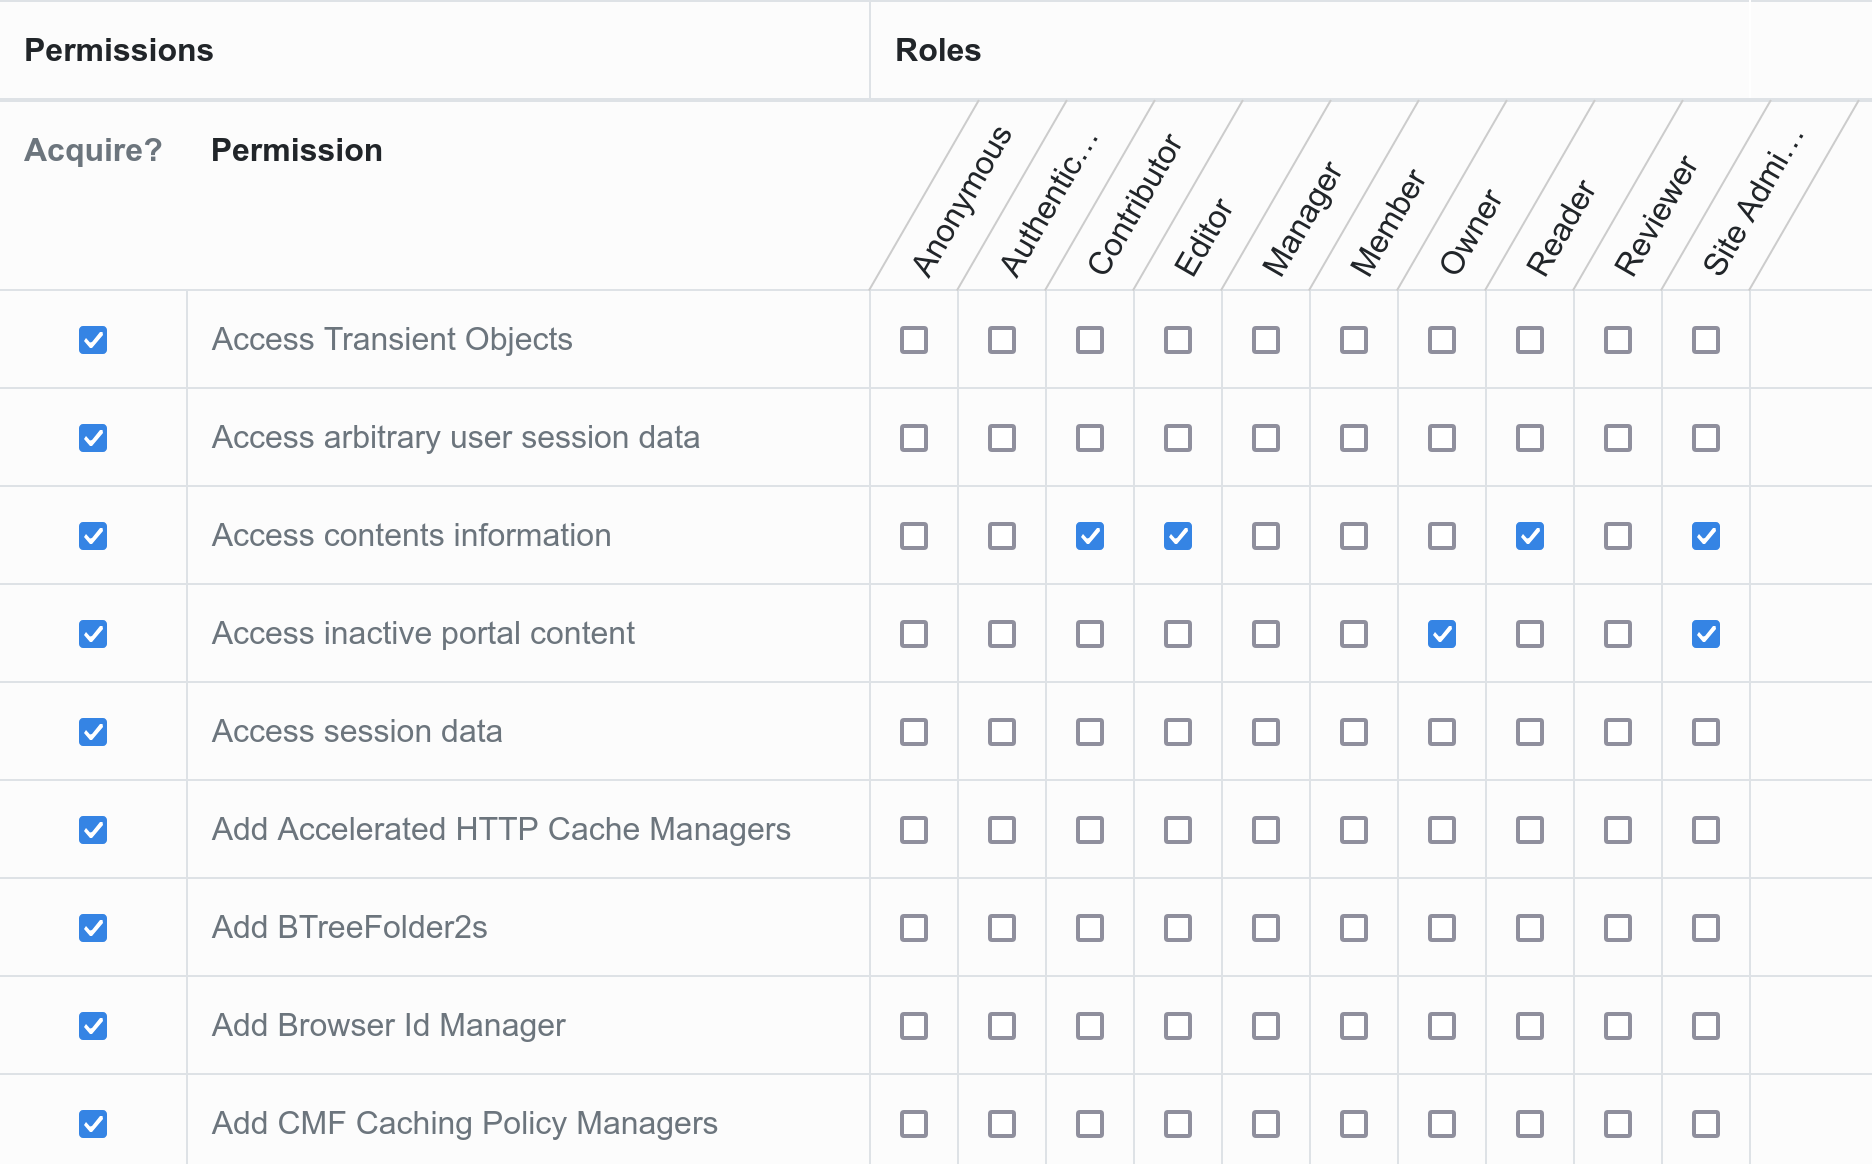
\includegraphics[width=0.95\columnwidth]{images/rolemap.png}
\end{frame}

%---------------------------------------------------------------------------------------

\begin{frame}{Hierarchical Object Database}
  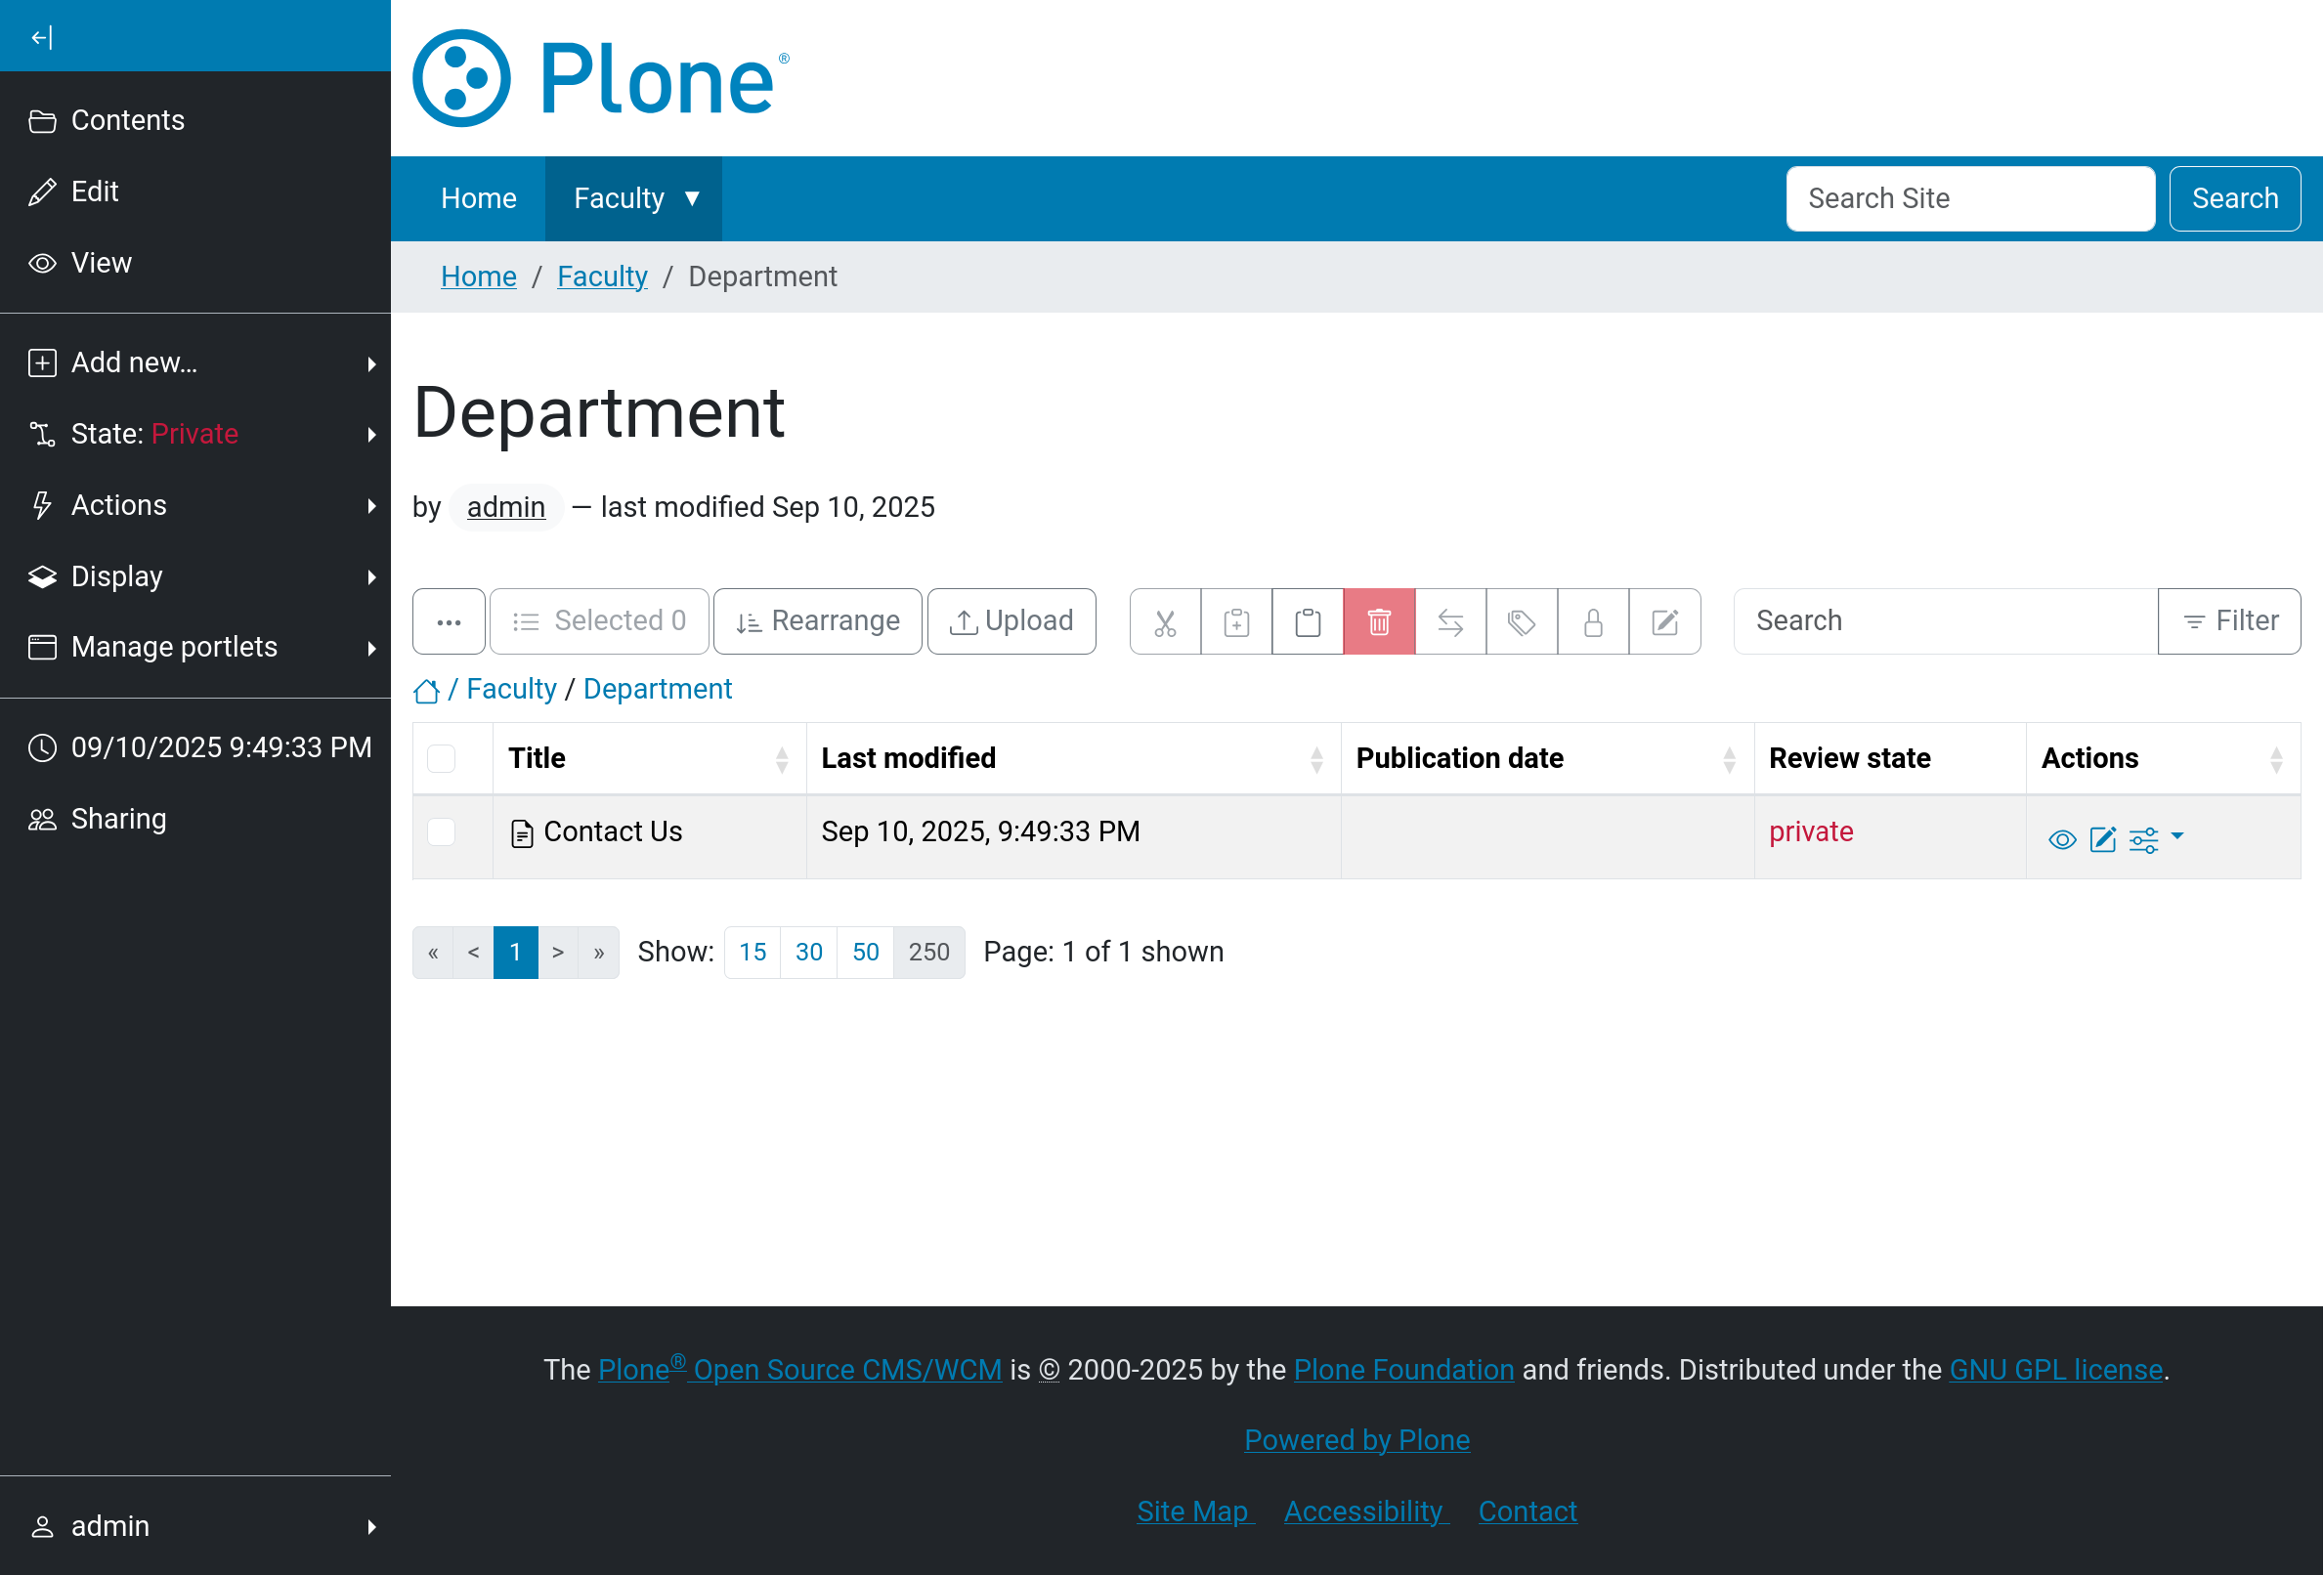
\includegraphics[width=1\columnwidth]{images/contents.png}
\end{frame}

%---------------------------------------------------------------------------------------

\begin{frame}{Types}
  \begin{columns}
    \begin{column}{0.3\textwidth}
      \begin{itemize}
        \item Fieldsets
        \item Fields
        \item Widgets
        \item Options
        \item "Behaviors"
        \item Subtypes
      \end{itemize}
    \end{column}
    \begin{column}{0.35\textwidth}
      \centering
      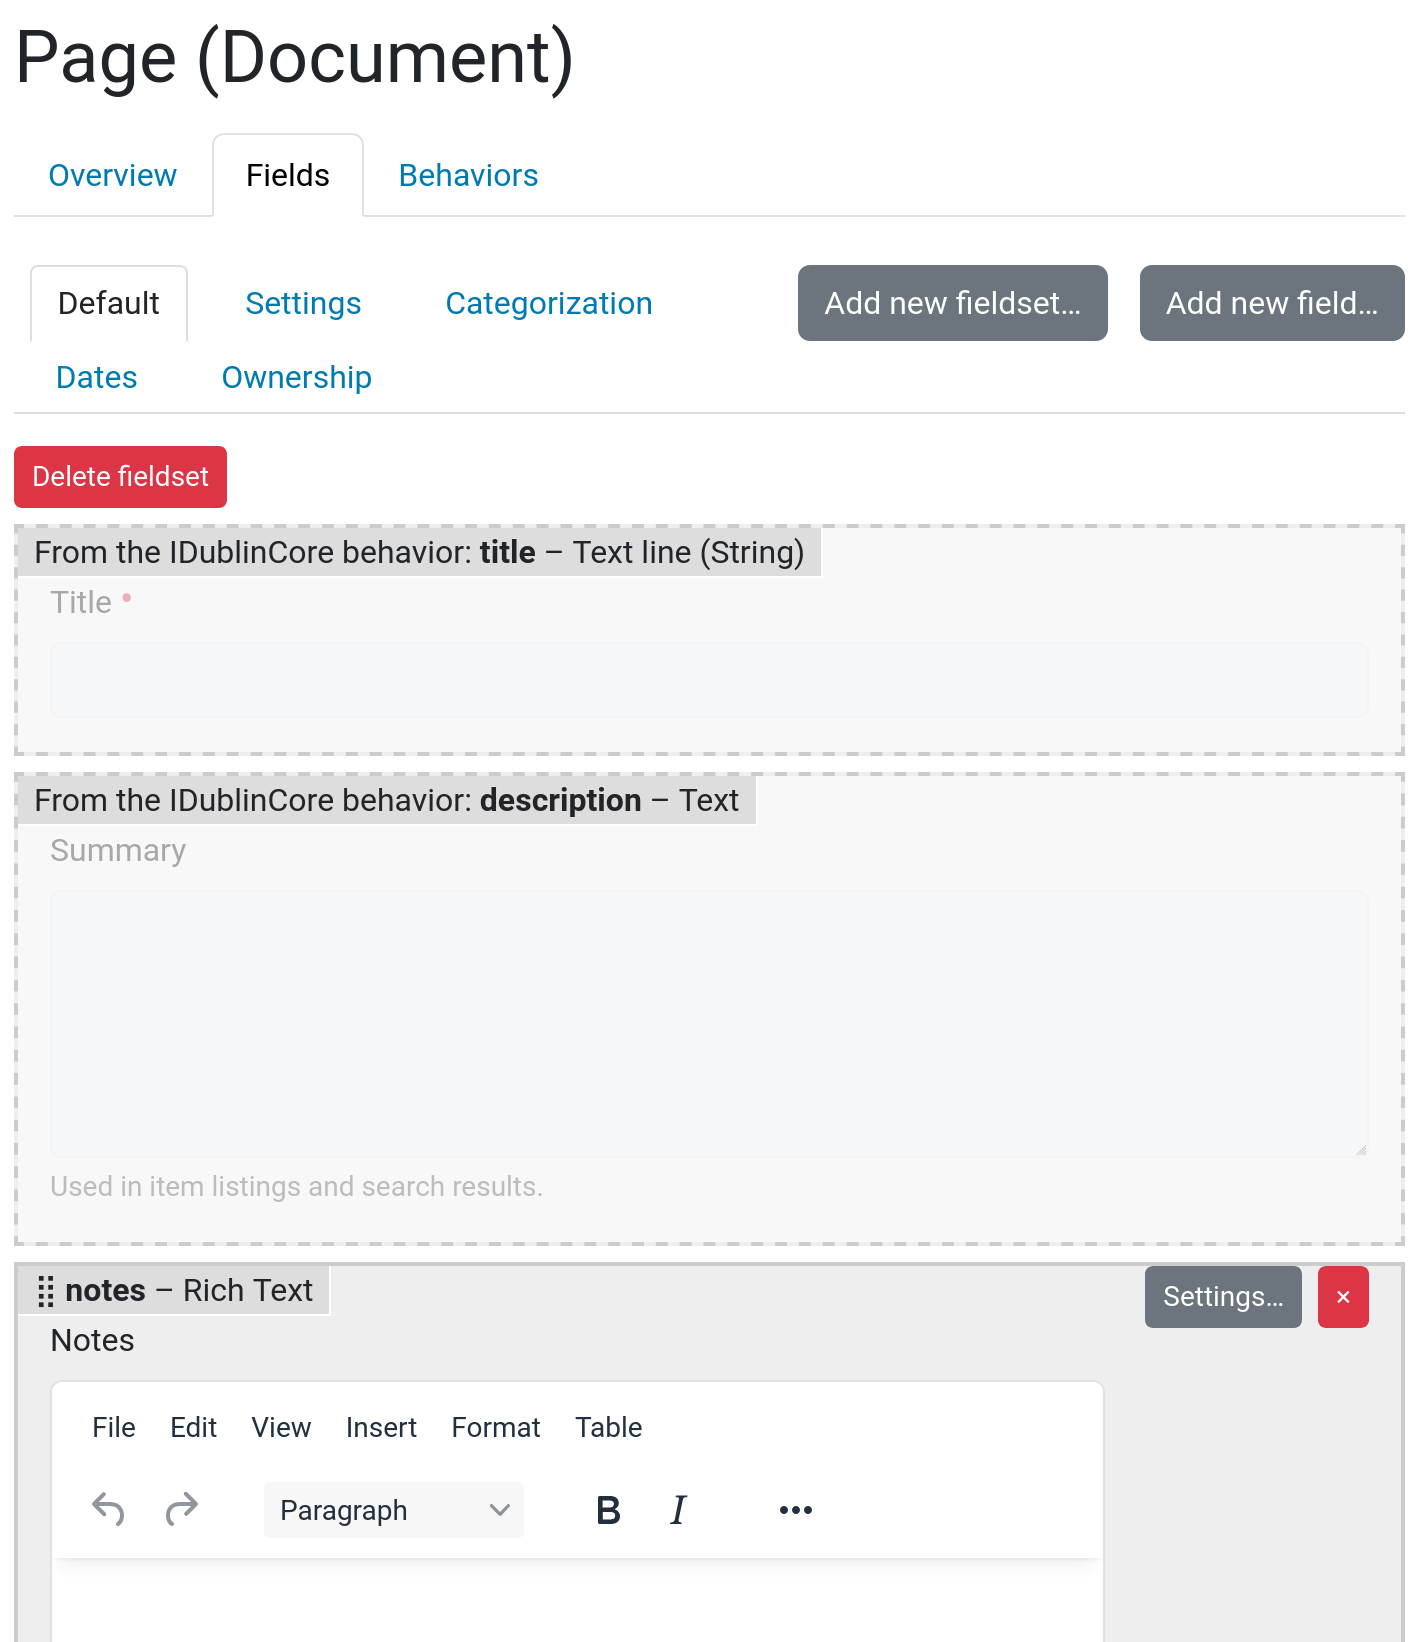
\includegraphics[width=0.95\columnwidth]{images/dexterity-01.png}
    \end{column}
    \begin{column}{0.35\textwidth}
      \centering
      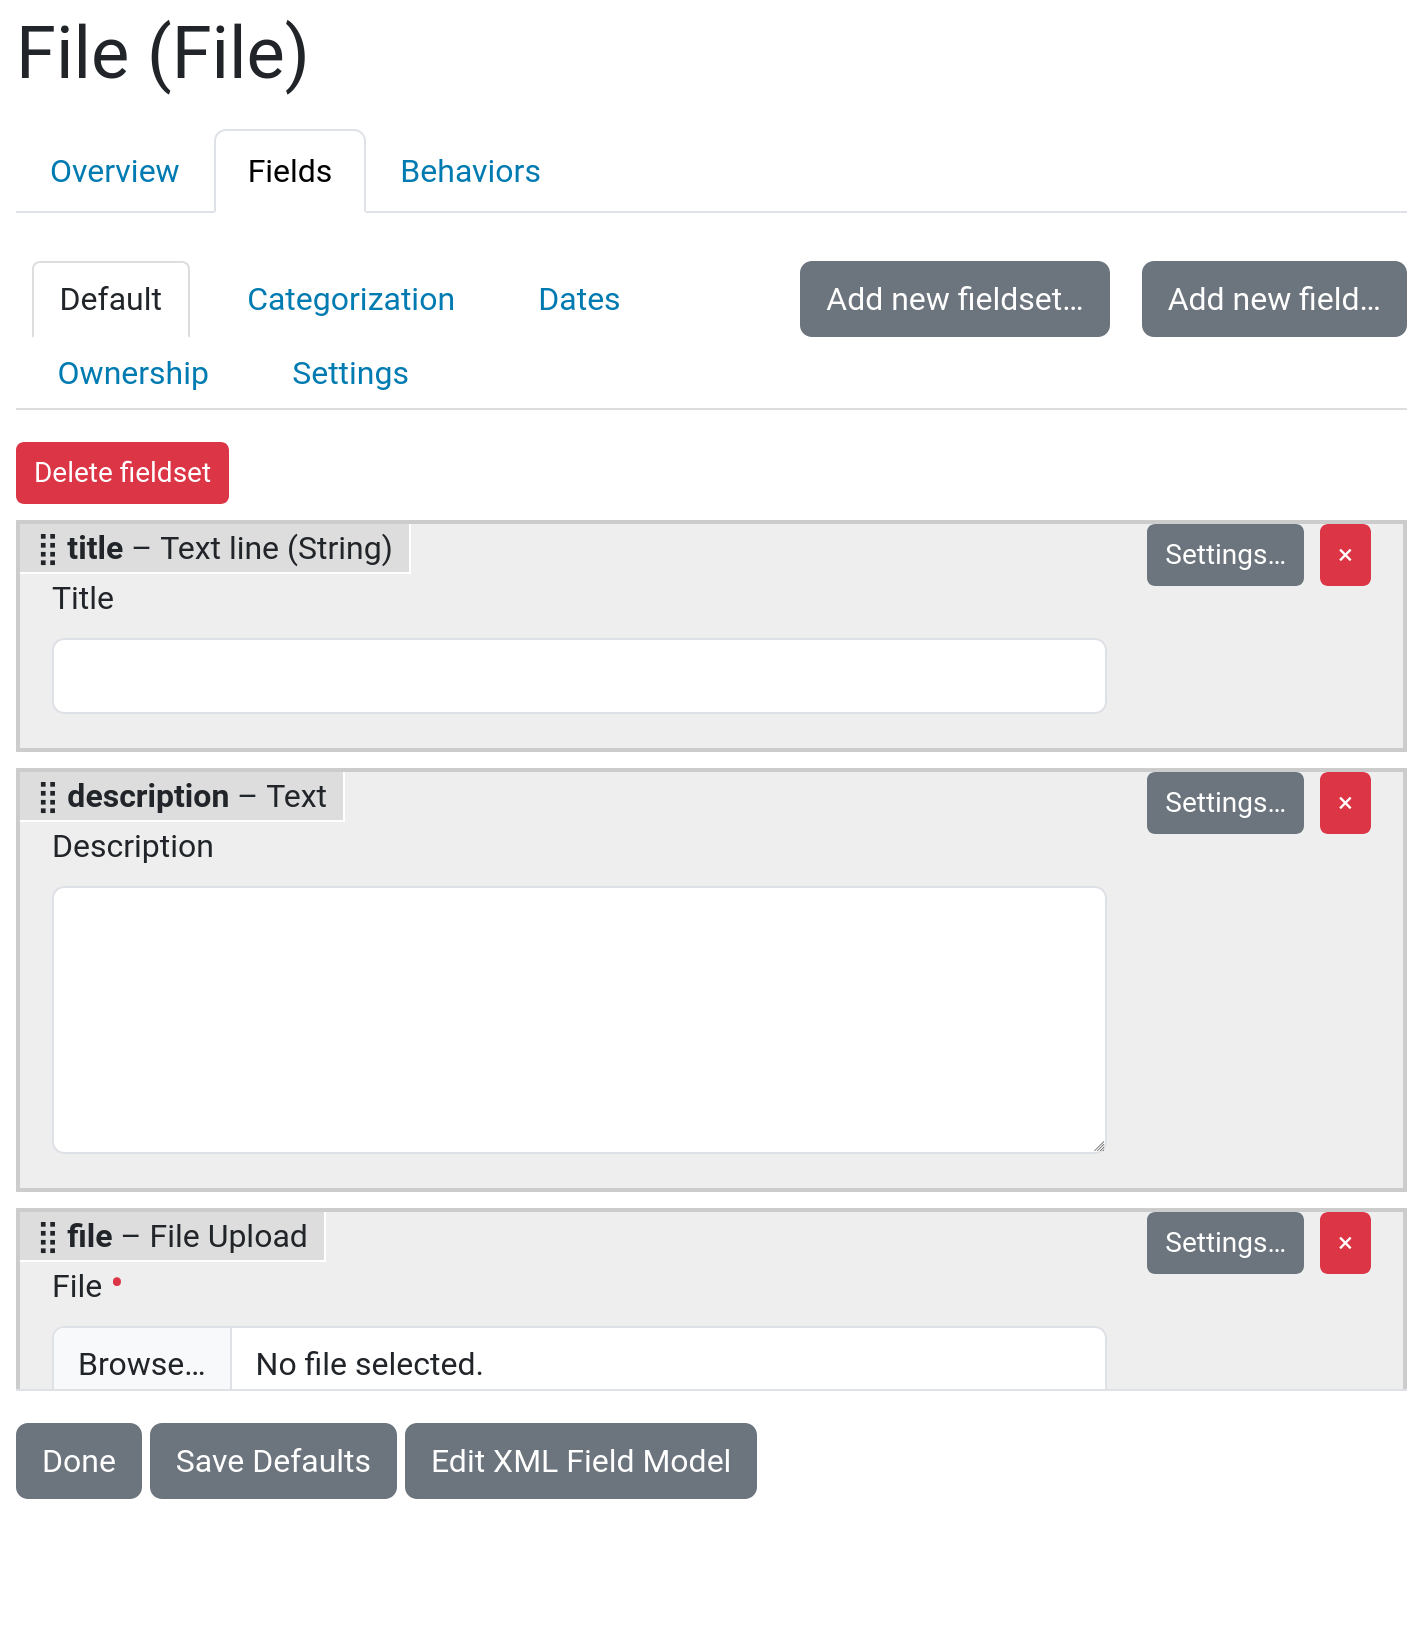
\includegraphics[width=0.95\columnwidth]{images/dexterity-02.png}
    \end{column}
  \end{columns}
\end{frame}

%---------------------------------------------------------------------------------------

\begin{frame}{Content Rules}
  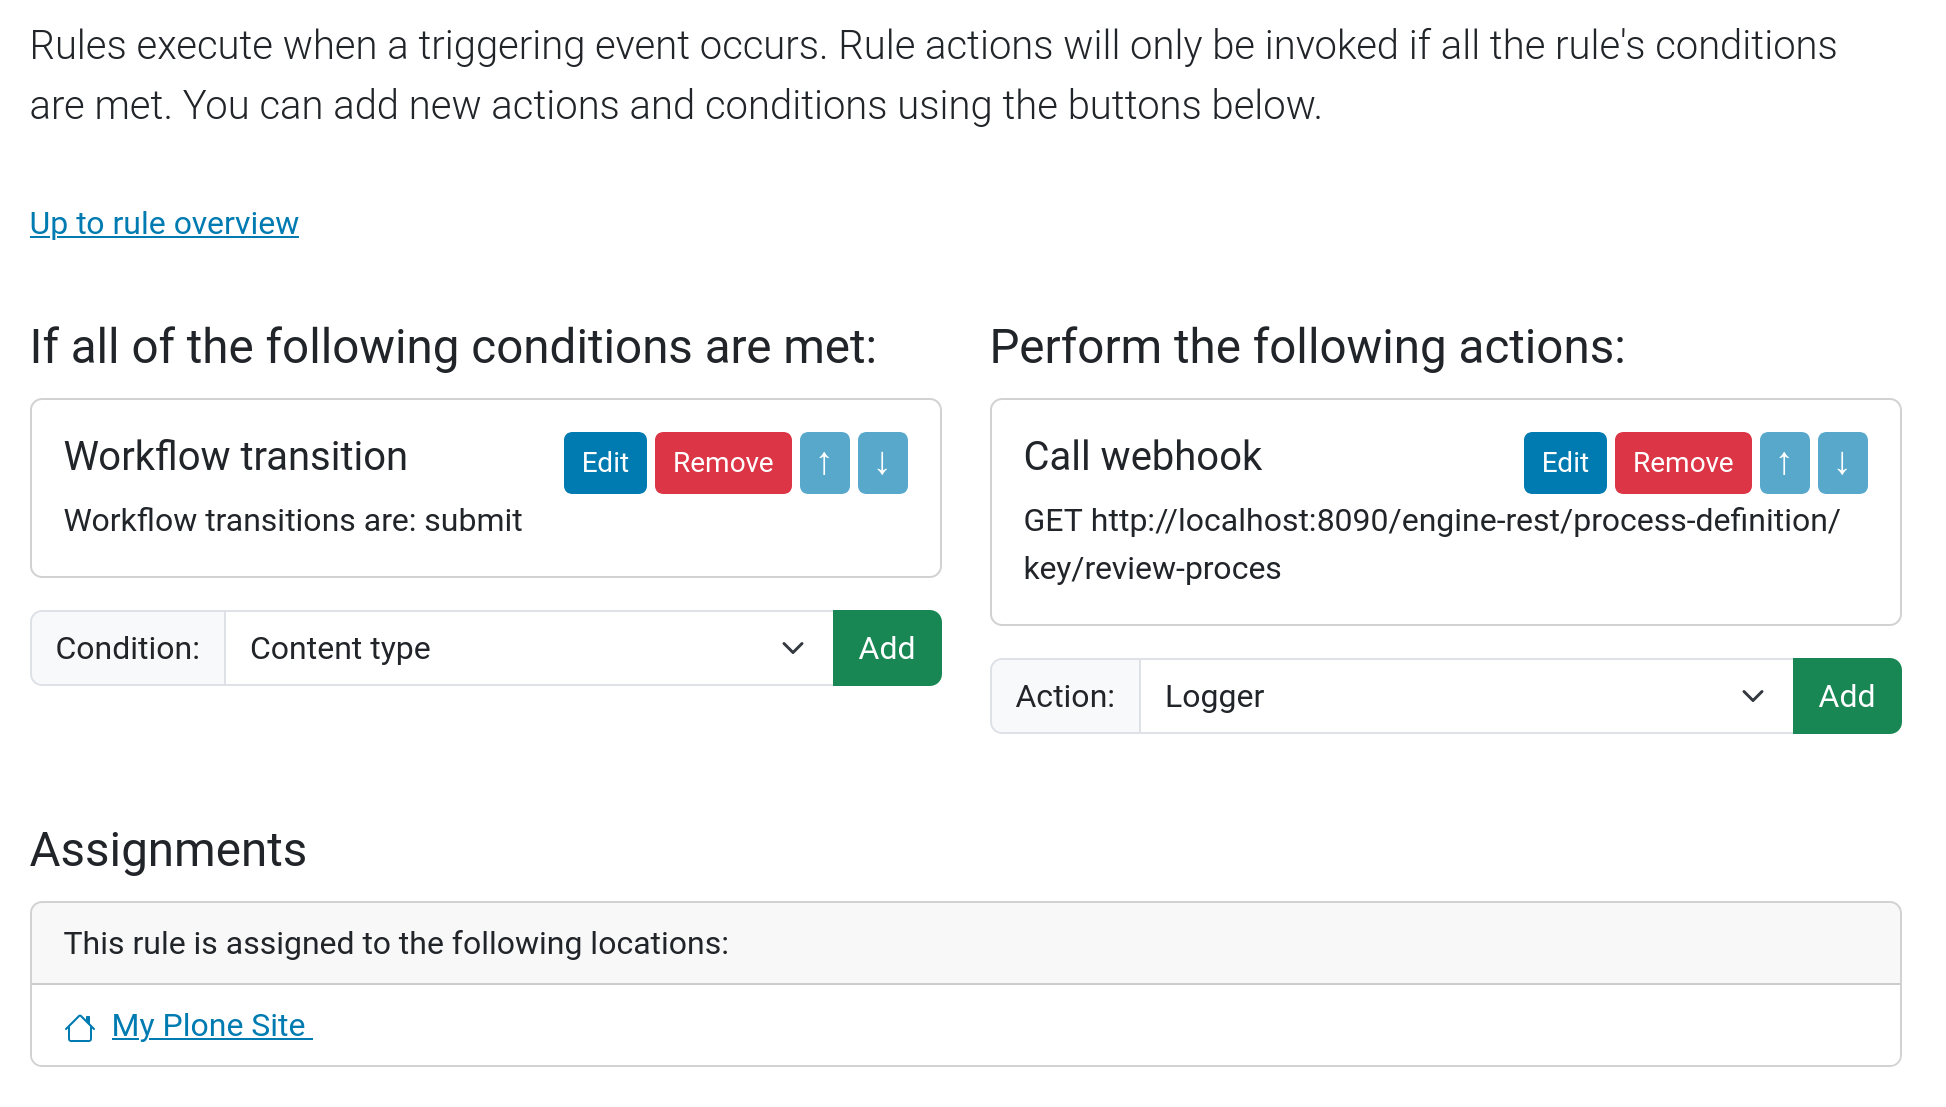
\includegraphics[width=0.95\columnwidth]{images/content-rules.png}
\end{frame}

%---------------------------------------------------------------------------------------

\begin{frame}[fragile]{Plone 7: Headless UI}
\tiny
\begin{minted}{jsx}
import { useQuery } from '@tanstack/react-query';
import ploneClient from '@plone/client';

const client = ploneClient.initialize({
  apiPath: 'http://localhost:8000',
});

function App() {
  const { getContentQuery } = client;
  const { data: content, isLoading } = useQuery(getContentQuery({ path: '/' }));

  return (
    <div>
      {!!isLoading && content && (
        <article>
          <h2>{content.title}</h2>
          {content.description && <p>{content.description}</p>}
        </article>
        )
      )}
    </div>
  );
}

export default App;
\end{minted}
\end{frame}

%---------------------------------------------------------------------------------------

\begin{frame}[fragile]{Plone 7: Headless UI}
  
\includegraphics[width=0.95\columnwidth]{images/vite.png}
\end{frame}

%---------------------------------------------------------------------------------------

\begin{frame}{Plone CMS with BPMN driven orchestration}
\centering
\begin{tikzpicture}[every node/.style={font=\sffamily}]
  % REST API box
  \node[draw, thick, rounded corners, fill=none, minimum width=6.2cm, minimum height=3.5cm, label=above:{REST API}] (restapi) {};
  % Headless CMS box inside REST API
  \node[draw, thick, fill=blue!10, minimum width=4.8cm, minimum height=2.2cm] (cms) at (restapi.center) {};
  % Content inside CMS
  \node[draw, fill=red!10, minimum width=3.0cm, minimum height=0.9cm] (content) at (cms.center) {\footnotesize Backend / Classic};

  % External components
  \node[draw, fill=red!10, minimum width=3.5cm, minimum height=0.7cm] (presentation) at ([yshift=-1cm]restapi.south) {\footnotesize Frontend / Volto};
  \node[draw, fill=red!10, minimum width=3.5cm, minimum height=0.7cm, anchor=west] (process) at ([xshift=1.2cm]restapi.east) {\footnotesize Operaton BPM};
  \node[draw, fill=red!10, minimum width=3.5cm, minimum height=0.7cm, anchor=north] (integrations) at ([xshift=0cm,yshift=-0.7cm]process.south) {\footnotesize Microservices};

  % Bidirectional arrows (external components <-> REST API)
  \draw[<->, thick] (presentation.north) -- (restapi.south);
  \draw[<->, thick] (process.west) -- (restapi.east);
  \draw[<->, thick] (integrations.north) -- (process.south);
  \draw[<->, thick] (integrations.west) -- ([yshift=-1.4cm]restapi.east);
\end{tikzpicture}
\end{frame}


%---------------------------------------------------------------------------------------

\begin{frame}
\vfill
\huge
\centering 
\includegraphics[height=0.50\paperheight]{images/PyCon-Finland.pdf}
\par
\textbf{\href{https://pyconfi.ploneconf.org}{fi.pycon.org}}
\par
\normalsize
\vfill
PyCon Finland 2025 – Friday, October 17th – Jyväskylä \\
\vfill
\end{frame}

\end{document}

